\section{Register Stack}

Actually, the local registers in MMIX are more complicated than explained at the beginning. Because MMIX uses a combination of registers and memory for the stack. This way, \glslink{Subroutine linkage}{subroutine linkage} is realized. Additionally, MMIX offers instructions to save or restore the complete state of a running program using the stack. Both are explained in detail in this section.

\subsection{Subroutine Linkage}

Because of the complexity of the \glslink{Subroutine linkage}{subroutine linkage} mechanism, it is explained in two steps. At first, it is shown from the perspective of the programmer. Afterwards the internal functional principle is described.

\subsubsection{Programmers View}

The programmer has \sr{G} local registers named \dr{0}, \dots, \dr{(\sr{G} - 1)} at his hand. The registers \dr{0}, \dots, \dr{(\sr{L} - 1)} are the currently used ones, while \dr{(\sr{L})}, \dots, \dr{(\sr{G} - 1)} are the marginal registers. Furthermore he can think of the stack as an potentially unbounded list $S$. The stack pointer, \ie the pointer that indicates the slot in $S$ that is going to be written next, is called $\tau$, which is initially zero. \citep[pg. 22]{mmix-doc}

\paragraph{Calling and Returning}

MMIX provides two instruction families to call subroutines and return from them.

\instrtblseven
	{\mi{PUSHJ \$X,@+4*(YZ[-$2^{16}$]),\quad PUSHGO \$X,\$Y,\$Z|Z}}
	{$S[\tau] \leftarrow \dr{0}, S[\tau+1] \leftarrow \dr{1}, \dots, S[\tau + {\tt X} - 1] \leftarrow \dr{(X - 1)}$}
	{$S[\tau + {\tt X}] \leftarrow {\tt X}$}
	{$\tau \leftarrow \tau + {\tt X} + 1$}
	{$\dr{0} \leftarrow \dr{X + 1}, \dr{1} \leftarrow \dr{X + 2},\dots, \dr{(\sr{L} - X - 2)} \leftarrow \dr{(\sr{L} - 1)}$}
	{$\sr{L} \leftarrow \sr{L} - {\tt X} - 1$}
	{$\sr{J} \leftarrow @ + 4$}
	{$@ \leftarrow (@+4*({\tt YZ}[-2^{16}]))~|~(\dr{Y} + \udrim{Z})$}
\noindent At first, \mi{PUSHJ} (\i{push registers and jump}) and \mi{PUSHGO} (\i{push registers and go}) are essentially the same, except that MMIX determines the new value of the \glslink{PC}{instruction pointer} in different ways. The first action they perform is to push the current local registers \dr{0}, \dots, \dr{(X - 1)} onto the stack $S$. Afterwards the number of registers, that have been \i{pushed down}, is saved in $S[\tau + {\tt X}]$ and $\tau$ is increased correspondingly. The next step is to rename the current registers \dr{(X + 1)}, \dots, \dr{(\sr{L} - 1)} to \dr{0}, \dots, \dr{(\sr{L} - X - 2)}. That means, all used registers above {\tt X} are passed as arguments to the subroutine, where they appear as \dr{0}, \dr{1} and so on. Finally, \sr{L} is adjusted, so that only the arguments are currently in use, the \i{return-jump register} \sr{J} is set to the instruction that would have been executed normally and the \glslink{PC}{instruction pointer} is changed. \citep[pg. 22]{mmix-doc}

\instrtblseven
	{\mi{POP X,YZ}}
	{$x \leftarrow S[\tau - 1] \bmod 256$}
	{$S[\tau - 1] \leftarrow \dr{(X - 1)}$}
	{$\sr{L} \leftarrow min(x + {\tt X},\sr{G})$}
	{$\dr{(\sr{L} - 1)} \leftarrow \dr{(\sr{L} - x - 2)}, \dots \dr{(x + 1)} \leftarrow \dr{0}$}
	{$\dr{x} \leftarrow S[\tau - 1], \dr{(x - 1)} \leftarrow S[\tau - 2], \dots, \dr{0} \leftarrow S[\tau - x - 1]$}
	{$\tau \leftarrow \tau - x - 1$}
	{$@ \leftarrow \sr{J} + 4*{\tt YZ}$}
\noindent Of course, \mi{POP} (\i{pop registers and return from subroutine}) basically behaves in the opposite way as \mi{PUSHJ} and \mi{PUSHGO} do. At first, the number of registers that have been pushed down by the associated \mi{PUSHJ} or \mi{PUSHGO} are loaded from $S[\tau - 1]$. It can not be more than 255, because MMIX has only 256 dynamic registers. In the next step, MMIX sets $S[\tau - 1]$ to the "main return value" \dr{(X - 1)}, which is used later. Next, \sr{L} is adjusted to be the number of local registers the caller wanted to keep plus the number of return values, denoted by {\tt X}. Of course, that should not be more than \sr{G}. Subsequently, the registers holding the return values (except the main return value) are renamed, so that they appear in \dr{(x + 1)}, \dots, \dr{(\sr{L} - 1)} for the caller. Finally, the previously saved values are restored from the stack, $\tau$ is adjusted correspondingly and MMIX jumps back to the location stored in \sr{J}. Optionally, some instructions can be skipped with ${\tt YZ} > 0$. It is noteworthy that the main return value appears in the so called \i{hole} \dr{x}, \ie the register that has stored the number of registers that have been pushed down. \citep[pg. 22,23]{mmix-doc}

\paragraph{Example}

To make the just described instructions more clear, the following goes through an example. It supposes, that the first four local registers have some values and a \mi{PUSHJ \$1,Sub} is executed. The following figure illustrates the state before the \mi{PUSHJ} and the state afterwards, \ie the initial state in subroutine \i{Sub}:
\begin{figure}[H]
	\centering
	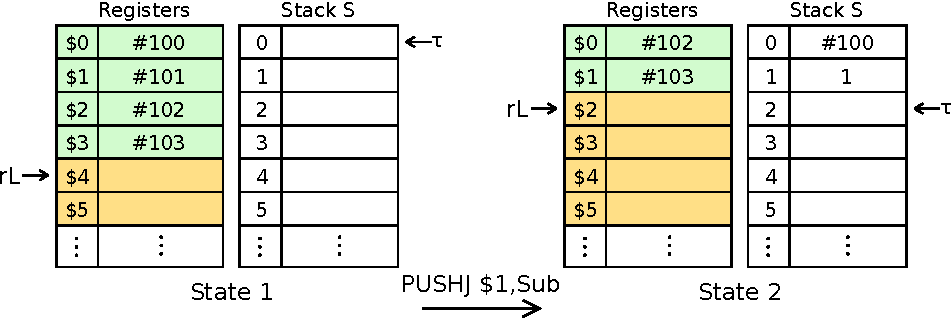
\includegraphics[width=\textwidth]{img/push-pop-user1-crop.pdf}
	\caption{Register stack: User perspective, state 1 to 2}
	\label{figure:push-pop-user1}
\end{figure}
\noindent The figure displays the used local registers green and the marginal ones orange. At first \dr{0} and \dr{1} are saved on the stack, whereas \dr{1} has been set to the number of pushed down values. Afterwards \dr{2} and \dr{3} are pushed as arguments to \i{Sub}, appearing as \dr{0} and \dr{1}. Thus, \sr{L} is 2 and $\tau$ is 2 as well.

In the next step of the example \i{Sub} performs some calculations, leading to state 3, and executes a \mi{POP 4,0} to return to the caller, whose state is shown on the right:
\begin{figure}[H]
	\centering
	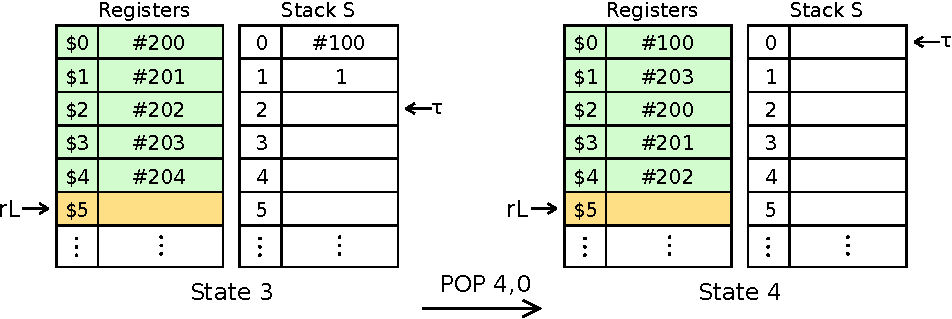
\includegraphics[width=\textwidth]{img/push-pop-user2-crop.pdf}
	\caption{Register stack: User perspective, state 3 to 4}
	\label{figure:push-pop-user2}
\end{figure}
\noindent As the figure shows, \dr{0}, \dots, \dr{4} have been set to some arbitrary values. The subsequent \mi{POP 4,0} at first loads the number of pushed down registers from the stack, \ie $S[\tau - 1] = 1$. Based on that, it restores \haddr{100} from $S[0]$ into \dr{0}, sets the hole (\dr{1}) to the last return value \haddr{203} and \dr{2}, \dots, \dr{4} to the other return values in the original order. Thus, \sr{L} is $1+{\tt X} = 5$ and $\tau$ is zero again.

At this point it might look strange that the last return value appears first for the caller, followed by the other ones in the same order they were in the registers of \i{Sub}. The section about the internal view will show the reason for that behaviour.

\paragraph{Special Cases}

Unfortunatly it is even more complicated as just described, because some special cases have been suppressed. The instructions \mi{PUSHJ|PUSHGO \$X,\dots} have the following special cases:
\begin{itemize}
	\item If $\sr{L} \le {\tt X} < \sr{G}$, the value of \sr{L} will be increased to ${\tt X} + 1$ first.
	\item If ${\tt X} \ge \sr{G}$, all local registers \dr{0}, \dots, \dr{(\sr{L} - 1)} will be saved, followed by \sr{L} and \sr{L} will be reset to zero.
\end{itemize}
On the other hand, \mi{POP X,YZ} has to take care of:
\begin{itemize}
	\item If ${\tt X} > \sr{L}$, {\tt X} will be replaced by $\sr{L} + 1$ first and the hole will be set to zero.
	\item If ${\tt X} = 0$, the hole will disappear, \ie it will become marginal.
\end{itemize}
\citep[pg. 22,23]{mmix-doc}

\subsubsection{Internal View}

After having described the procedure of calling subroutines and returning from them from the perspective of the programmer, it should be explained how MMIX does actually achieve that.

As mentioned previously, MMIX has a local register array $l$ with either 256, 512 or 1024 slots. It is used as a ring, which means that if we have the local registers $l[0]$, $l[1]$, \dots, $l[255]$, register $l[256]$ will be the same as $l[0]$, $l[257]$ the same as $l[1]$ and so on.

To realize the register stack, MMIX has to manage the registers and the stack in memory. To do so, the register ring is divided into three parts by $\alpha$, $\beta$ and $\gamma$. $l[\alpha]$, $l[\alpha+1]$, \dots, $l[\beta-1]$ are corresponding to \dr{0}, \dr{1}, \dots, \dr{(rL - 1)}. The registers $l[\beta]$, \dots, $l[\gamma-1]$ are currently unused and $l[\gamma]$, \dots, $l[\alpha-1]$ are the registers that are currently not accessible, called \i{hidden}, but have not yet been stored to memory. The situation on the stack in memory is described by the special registers \sr{O} and \sr{S}. The former is the offset of \dr{0} in memory, \ie the location it would be written to. The latter is the location the next register is going to be written to. $\alpha$, $\beta$ and $\gamma$ relate to \sr{O} and \sr{S} in the following way (when $2^n$ is the number of slots in $l$):
$$\rm\alpha=(rO/8)\bmod2^n,\qquad \beta=(\alpha+rL)\bmod2^n,\qquad
\hbox{and}\qquad \gamma=(rS/8)\bmod2^n$$

To make sure that no value is lost, MMIX has to take care that $\alpha$, $\beta$ and $\gamma$ never move past each other. Whenever a \mi{PUSHJ|PUSHGO} is done, $\alpha$ moves towards $\beta$. Setting \dr{X} with ${\tt X} \ge \sr{L}$ means that \sr{L} is increased, \ie $\beta$ is moved towards $\gamma$. If $\beta$ moved past $\gamma$, registers would have to be written to memory first to free as many slots as required. To do so, $l[\gamma]$ is written to \vmem{8}{\sr{S}} and $\gamma$ is increased by one and thus \sr{S} by 8, until the new $\beta$ is less than $\gamma$. When doing a \mi{POP}, $\alpha$ moves backwards to $\gamma$. If this moved $\alpha$ past $\gamma$, we would have to load values back from memory first. That means, $\gamma$ and \sr{S} are decreased and \vmem{8}{\sr{S}} is put into $l[\gamma]$ until the new $\alpha$ is less than $\gamma$. \citep[pg. 33]{mmix-doc}

The following figures illustrate the actions with a similar example as in the previous section. For simplicity it is assumed that only 4 local registers are present\footnote{This is not specification conform, as explained previously, but simplifies the example.}:
\begin{figure}[H]
	\centering
	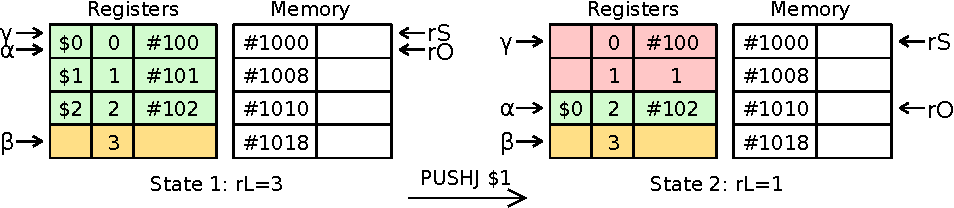
\includegraphics[width=\textwidth]{img/push-pop-internal1-crop.pdf}
	\caption{Register stack: Internal perspective, state 1 to 2}
	\label{figure:push-pop-internal1}
\end{figure}
\noindent The green and yellow cells have the same meaning as in figures \ref{figure:push-pop-user1} and \ref{figure:push-pop-user2}, while the red cells are the hidden registers. The register block on the left shows the current assignment of dynamic registers, the local register index and the value in the register. The right block displays the stack in memory with the address and the value. Additionally the values of $\alpha$, $\beta$, $\gamma$, \sr{O} and \sr{S} are indicated by pointing to the corresponding register or memory slot.

In the first state, three registers are used, $\alpha$ and $\gamma$ are zero, $\beta$ is $\alpha+\sr{L} = 3$ and \sr{O} and \sr{S} have the value \haddr{1000}. State 2 is reached by doing a \mi{PUSHJ \$1}. Hence, the offset $\alpha$ in the register ring is increased by 2 and the offset \sr{O} in memory is increased by 16. Additionally, the hole ($l[1]$) is set to the number of registers that have been pushed down.

\begin{figure}[H]
	\centering
	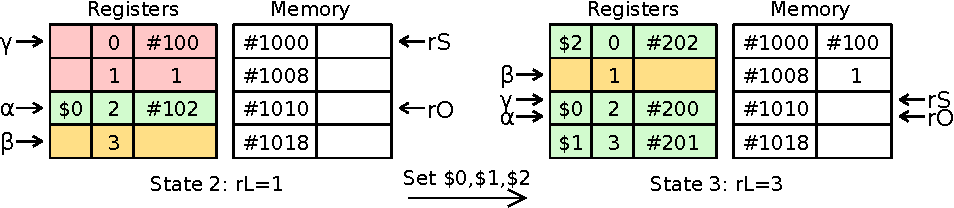
\includegraphics[width=\textwidth]{img/push-pop-internal2-crop.pdf}
	\caption{Register stack: Internal perspective, state 2 to 3}
	\label{figure:push-pop-internal2}
\end{figure}
\noindent The third state, shown in figure \ref{figure:push-pop-internal2}, is reached by setting \dr{0}, \dr{1} and \dr{2} to \haddr{200}, \haddr{201} and \haddr{202}, respectively. Setting \dr{0} does not increase \sr{L}, so that only $l[2]$ is changed. The other two both increase \sr{L} by one, \ie move $\beta$ towards $\gamma$. Thus, in each case $\gamma$ and \sr{S} are increased and a value is written to memory.

\begin{figure}[H]
	\centering
	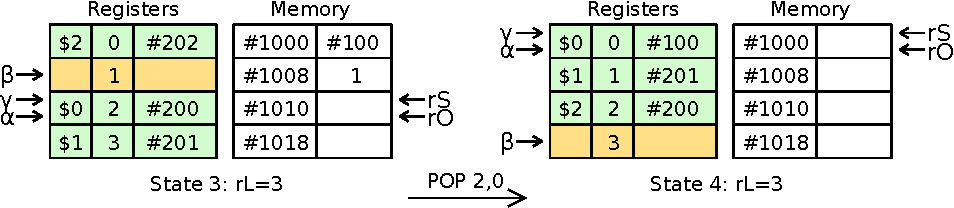
\includegraphics[width=\textwidth]{img/push-pop-internal3-crop.pdf}
	\caption{Register stack: Internal perspective, state 3 to 4}
	\label{figure:push-pop-internal3}
\end{figure}
\noindent The last transition, illustrated in figure \ref{figure:push-pop-internal3}, is achieved by doing a \mi{POP 2,0}. As described, \mi{POP} moves $\alpha$ back. The hole tells MMIX how many registers have been pushed down by the preceding \mi{PUSHJ} or \mi{PUSHGO}. In this case, the hole has been written to memory, so that it has to be loaded back first. Afterwards MMIX has to move $\alpha$ two steps up because one register has been saved and the hole has been created. To be able to decrease $\alpha$ and \sr{O}, one further value has to be loaded from memory. To return the two values, a move of $l[3]$ to $l[1]$ is sufficient because the other value is already in the desired slot (as all other return values would be, if there were more than two). This is the reason for the -- at a first glance -- strange order of the return values.

\subsection{Saving and Restoring the State}

Another concept, that works with the register stack as well, is the procedure of storing and restoring the state of the running program. It is intended both for the operating system and user applications. The former may use it for example to implement process switching or to save the state when handling an \glslink{Interrupt}{interrupt}. The latter can use it to implement thread switching in user space, for example.

\instrtblsix
	{\mi{SAVE \$X}}
	{$S[\tau{\tt ++}] \leftarrow \dr{0}, \dots, S[\tau{\tt ++}] \leftarrow \dr{(\sr{L} - 1)}$}
	{$S[\tau{\tt ++}] \leftarrow \sr{L}, \quad \sr{L} \leftarrow 0$}
	{$S[\tau{\tt ++}] \leftarrow g[\sr{G}], \dots, S[\tau{\tt ++}] \leftarrow g[255]$}
	{for $s \in \{\sr{B},\sr{D},\sr{E},\sr{H},\sr{J},\sr{M},\sr{R},\sr{P},\sr{W},\sr{X},\sr{Y},\sr{Z},(\sr{G} \ll 56) \lor \sr{A}\}$}
	{$\quad S[\tau{\tt ++}] \leftarrow s$}
	{$\dr{X} \leftarrow \tau$}
\noindent Put simply, \mi{SAVE} (\i{save process state}) stores all registers that might affect the computation on the stack and writes the address of the topmost octabyte on the stack into \dr{X}. In detail, it means that at first all hidden registers are written to memory (which is not listed in the effect description, because it shows it from the programmer perspective). Afterwards all used local registers are written behind them, followed by \sr{L} and \sr{L} is set to zero. In the next step, all global registers are written to memory, followed by the special registers that affect the computation, whose last value is an octabyte containing \sr{G} in the most significant byte and \sr{A} in the least significant ones. As will be described shortly, the value of \dr{X} after executing \mi{SAVE \$X} can be used for \mi{UNSAVE}. \citep[pg. 34]{mmix-doc}

\instrtblsix
	{\mi{UNSAVE \$Z}}
	{$\tau \leftarrow \dr{Z}$}
	{for $s \in \{(\sr{G} \ll 56) \lor \sr{A},\sr{Z},\sr{Y},\sr{X},\sr{W},\sr{P},\sr{R},\sr{M},\sr{J},\sr{H},\sr{E},\sr{D},\sr{B}\}$}
	{$\quad s \leftarrow S[{\tt --}\tau]$}
	{$g[255] \leftarrow S[{\tt --}\tau], \dots, g[\sr{G}] \leftarrow S[{\tt --}\tau]$}
	{$\sr{L} \leftarrow S[{\tt --}\tau]$}
	{$\dr{(\sr{L} - 1)} \leftarrow S[{\tt --}\tau], \dots, \dr{0} \leftarrow S[{\tt --}\tau]$}
\noindent Consequently, \mi{UNSAVE} (\i{restore process state}) goes the other way. It first sets the stack pointer to \dr{Z} and restores all special registers in the opposite order from the stack, followed by the global ones. Afterwards \sr{L} is loaded, that tells MMIX the number of local registers to restore from stack, which is done in the last step. \citep[pg. 34]{mmix-doc} It should be noted, that the hidden registers, that had been stored on the stack during \mi{SAVE} before the used local ones, are \i{not} restored by \mi{UNSAVE}. This is done by the next \mi{POP}, \ie as soon as they are needed.

